\section{Understanding Decision Trees}

A decision tree is one of the most intuitive and interpretable machine learning models used for both classification and regression tasks. In the context of climate analysis, decision trees help us understand how various atmospheric conditions contribute to an event such as heavy rainfall.


\subsection*{How Decision Trees Work}

A decision tree splits the dataset into branches based on the values of the input features. Each internal node represents a condition on a feature, and each leaf node represents an outcome.

The model continues to split the data into smaller groups to reduce uncertainty or “impurity.” In classification, a common measure for this impurity is the Gini Index or Entropy.

\begin{itemize}
  \item \textbf{Root Node:} The feature that best splits the data appears at the top.
  \item \textbf{Internal Nodes:} Represent decision rules based on features.
  \item \textbf{Leaf Nodes:} Represent class labels (e.g., 0 = No Heavy Rainfall, 1 = Heavy Rainfall).
\end{itemize}

\subsection*{Why Use Decision Trees in Climate Data?}

\begin{itemize}
  \item \textbf{Interpretability:} You can easily visualize and understand the rules that lead to predictions.
  \item \textbf{Non-linearity:} Trees can capture complex, non-linear interactions between variables.
  \item \textbf{No Need for Scaling:} Unlike many models, decision trees do not require feature standardization.
  \item \textbf{Handles Missing Values and Outliers:} Trees are robust to irregularities in the data.
\end{itemize}

\subsection*{Example Rule from the Tree}

Let’s say the decision tree discovers this rule: \\
If Humidity 2m $>$ 70 and Pressure $<$ 1010, then the model predicts Heavy Rainfall = 1.

This simple rule can help stakeholders quickly assess risk from available sensor readings.

\subsection*{Limitations of Decision Trees}

Despite their advantages, decision trees can overfit the training data if not carefully tuned. That means they may perform well on training data but poorly on unseen data. This can be mitigated by:

\begin{itemize}
  \item Pruning the tree (removing weak or unnecessary branches).
  \item Limiting the depth of the tree.
  \item Using ensemble methods (e.g., random forests or gradient boosting).
\end{itemize}

\subsection*{Visualizing the Tree Structure}

The tree diagram provides a clear representation of how the model splits the data and which features are most influential.

\begin{verbatim}
plot(tree_model)
text(tree_model, pretty = 0)
\end{verbatim}

This visualization not only shows the decision points but also helps explain the model’s logic to non-technical stakeholders, such as meteorologists or disaster management teams.

\subsection*{Classifying Heavy Rainfall Events Using Decision Trees}

To identify instances of heavy rainfall, we can use a decision tree model. In this section, we classify rainfall events as either Heavy or Not Heavy based on meteorological variables such as temperature, humidity, pressure, and wind speed.

We define a heavy rainfall event as one where precipitation exceeds the 75th percentile. The following R code demonstrates how to create and evaluate a decision tree model for this classification task.

\begin{verbatim}
# Install and load necessary package
install.packages("tree")
library(tree)
# Create a new column indicating heavy rainfall
precip_data <- climate_data %>%
  mutate(Heavy_Rainfall = ifelse(Precip > quantile(Precip, 0.75), 1, 0))
# Convert Heavy_Rainfall to factor for classification
precip_data$Heavy_Rainfall <- as.factor(precip_data$Heavy_Rainfall)
# Split data into training (80%) and testing (20%) sets
set.seed(123)
train_index <- createDataPartition(precip_data$Heavy_Rainfall, p = 0.8,
list = FALSE)
train_data <- precip_data[train_index, ]
test_data <- precip_data[-train_index, ]
# Train the decision tree model
tree_model <- tree(
Heavy_Rainfall ~ Temp_2m + Humidity_2m + Pressure + WindSpeed_10m, 
data = train_data)
# View summary of the model
summary(tree_model)
# Make predictions on test data
predictions <- predict(tree_model, test_data, type = "class")
# Evaluate the model using confusion matrix
conf_matrix <- table(Predicted = predictions, Actual = test_data$Heavy_Rainfall)
print(conf_matrix)
# Calculate performance metrics
accuracy <- sum(diag(conf_matrix)) / sum(conf_matrix)
precision <- conf_matrix[2, 2] / sum(conf_matrix[, 2])
recall <- conf_matrix[2, 2] / sum(conf_matrix[2, ])
f1_score <- 2 * (precision * recall) / (precision + recall)
# Print metrics
cat("Accuracy: ", accuracy, "\n")
cat("Precision: ", precision, "\n")
cat("Recall: ", recall, "\n")
cat("F1-score: ", f1_score, "\n")


\end{verbatim}

% Figure here---------------------------
\begin{figure}[h]
\centering
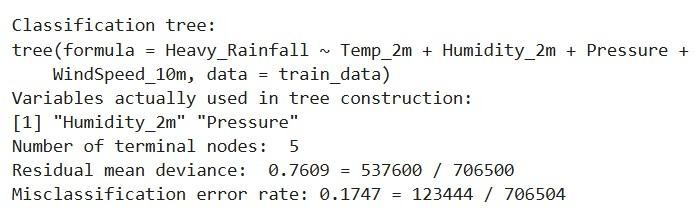
\includegraphics[width=0.5\textwidth]{figures/tree_summ.jpg}
\caption{Model summary}
\end{figure}

\begin{verbatim}
  # Visualize the decision tree
plot(tree_model)
text(tree_model, pretty = 0)
\end{verbatim}

% figure here----------------------------
\begin{figure}[h]
\centering
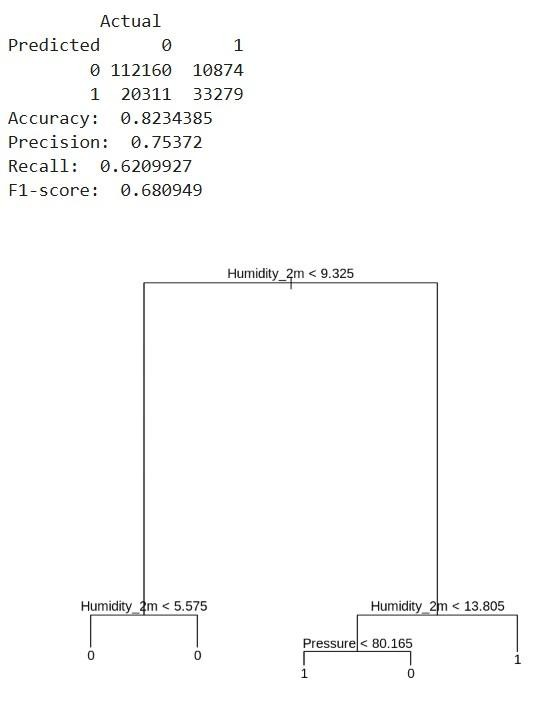
\includegraphics[width=0.5\textwidth]{figures/tree.jpg}
\caption{Classifying Heavy Rainfall Events Using Decision Trees}
\end{figure}

The decision tree model learns decision rules based on climate variables to classify whether a given observation is a heavy rainfall event.

The confusion matrix and the calculated performance metrics (accuracy, precision, recall, and F1-score) allow us to evaluate how well the model distinguishes between the two classes.

The visualization of the tree provides insight into which features most strongly influence the classification. This model can be improved or expanded by exploring ensemble techniques such as Random Forests or Gradient Boosting, which often provide more accurate and stable predictions.

\subsection*{Conclusion}

Decision trees offer a transparent and flexible way to classify rainfall events based on meteorological variables. When interpretability and ease of use are important, they can be an ideal choice in climate prediction applications.
